\usecasebase{Visualizzazione storico ordini}
\label{usecase:Storico ordini}

\begin{figure}[h]
	\centering
	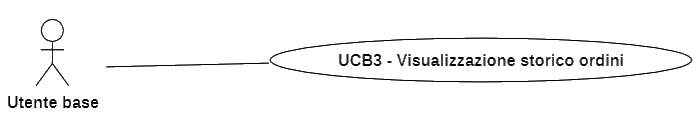
\includegraphics[width=0.8\textwidth]{./uml/UCB3.png} 
	\caption{Visualizzazione storico ordini}
	\label{fig:UCB3}
  \end{figure}

\begin{itemize}
	\item \textbf{Attore principale:} Utente base.

	\item \textbf{Precondizioni:}
	      \begin{itemize}
		      \item L'Utente ha eseguito correttamente l'accesso al Sistema come Utente base (vedi \autoref{usecase:Effettua accesso}).
		      \item L'utente deve trovarsi nella sua Area personale.
	      \end{itemize}

	\item \textbf{Postcondizione:} L'Utente base visualizza lo storico completo dei suoi ordini passati.

	\item \textbf{Scenario principale:}
	      \begin{enumerate}
		      \item Nella sezione Area personale, l'Utente base seleziona l'opzione per visualizzare lo storico dei suoi ordini;
		      \item Il Sistema presenta all'Utente base la lista degli ordini passati, ordinati cronologicamente dal più recente al meno recente.
	      \end{enumerate}
\end{itemize}

